
\chapter{Preliminaries}

In this chapter, I'll introduce the theoretical preliminaries needed to
understand the contributions and results of this paper. It is split into two main sections,
one on machine learning, and one on game theory. 

\section{Machine Learning}
Machine learning is the field of constructing algorithms that learn from data.
There are several subfields within machine learning. Within machine learning,
there is e.g. the supervised and unsupervised distinction. Unsupervised
learning tries to make sense of unannotated data, while supervised learning is
given the true answer to a problem and the inputs, and then tries to work out
how to solve the problem.

In our case, we are interested in supervised learning problems, since
these are the tasks we can sell off in analytics markets.

\subsection{Supervised Learning}
Within supervised learning, we have regression and classification. In
regression problems, we are looking to learn to find a numerical output based
on some input. In classification, we are instead trying to find a categorical
classification based on the input. Regression problems and classification
problems share many facets and are quite similar under the hood.

When understanding supervised learning, we often see our data as a table, known
as a tabular dataset. Here, every row is an observation, and every column is a
feature. For every row, a true label or class known as the target might be
attached, and a method can only be trained on rows where the label is available.
A tabular dataset is shown in figure \ref{fig:tab_data}.

\begin{figure}
  \centering
  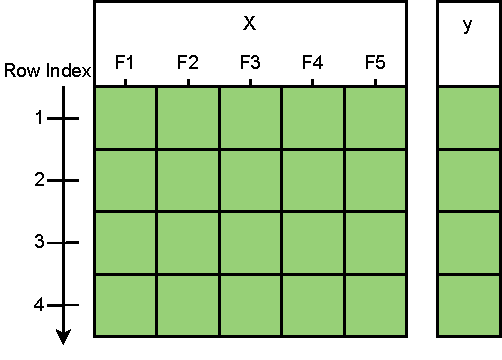
\includegraphics{Pictures/tabular_dataset.pdf}
  \caption{A diagram of a tabular dataset. Every green square is a single
  numerical or categorical value. The dataset has 5 columns and 4 rows, i.e. 5
  features and 4 observations. Attached to every row is also a true target, seen
  in the vector y.}
  \label{fig:tab_data}
\end{figure}

A supervised learning method generates based on every row indexed by $t$ a
prediction of the true label $\hat y_t$. It does this based on some function $f
: \mathcal X \rightarrow \mathcal Y$, where $\mathcal X$ is the space that the
features exist in or the \emph{feature space}, and $\mathcal Y$ is the space
that the targets exist in or the \emph{target space}. Then, predictions are made
as $\hat y_t = f(\mathbf{x}_t)$. The problem of supervised learning is really
the problem of making a "good" choice of function $f$, by some understanding of
the word good.

Features and targets can come from different spaces depending on the specific
regression problem. Very commonly features are continuous, in which case they
come from the real numbers, or a subset of the real numbers, but they can also
often be discrete in case of ordinal or cardinal features. Targets as well can
be continuous or discrete, in many different ways, e.g. $\mathcal Y = {0,1}$
for binary classification, $\mathcal Y = {0,1,2,..,K}$ for K-class
classification, or $\mathcal Y = \mathbb R$ for ordinary least squares
regression, to name a few.

Most supervised learning methods choose a function $f$ from a family of
functions $\mathcal F$ with some unknown parameters. To do this, we need to
decide what a "good" choice of function is.

\subsubsection{Maximum Likelihood Estimation}

We can model the relation between the features and targets as a joint
probability distribution.  This naturally lends a family of functions $f$,
namely the expected value of $y_t$ under the distribution, $f(x_t) = \mathbb E
\lbrack y | x_t \rbrack$. Determining the parameters of the probability
distribution will then also give us parameters for the function $f$. The
probability density function of the joint probability distribution is usually
denoted by $f$, but since $f$ is already in use, I'll denote it $g$. I will
also introduce the symbol $z$ which I use to denote an entire dataset
containing both $x$ and $y$. So $z_t$ is an observation of both $x_t$ and $y_t$
at time $t$, and the distribution $g$ is a distribution over $z$. TODO

To determine the parameters of the probability distribution, we can use the
\emph{likelihood function}. The likelihood function gives the probability of a
certain observation given the parameters $\theta \in \Theta$ of the joint
distribution. It is written

\begin{equation}
  \mathcal L(\theta | z) = g(z | \theta)
\end{equation}

where $g$ is the probability density function for the joint probability
distribution and $\theta$ is the parameters for the joint probability
distribution. We can estimate the parameters by finding the parameters that
maximize the likelihood function, which is known as the maximum likelihood
estimate, or MLE, for the parameters. This estimator has some nice properties,
it e.g. guarantees convergence to the estimated value as the sample size goes
to infinity TODO: SHOULD I HAVE MORE PROPERTIES?. Using the MLE estimator is a
solution for finding a "good" function to map from features to targets, since
once we estimate the parameters of the distribution, we can use the expected
value as our function $f$ as mentioned earlier.

Assuming that every observation $z_t$ is independent and identically
distributed, the likelihood function is the product of the likelihood for every
observation individually. This naturally leads us to take the take the
logarithm of the likelihood function, which turns out to be useful for more
reasons than just turning this product into a sum.

\begin{equation}
  \text{log} \mathcal L(\theta | z) = \text{log} \prod_t^T \mathcal L(\theta | z_t) = \sum_t^T \text{log} \mathcal L(\theta | z_t)
\end{equation}

Usually, it is more handy to maximize the log likelihood function, as we'll see
later in the regression subsection TODO:REF.

\subsubsection{Loss Functions}

The negative log-likelihood function naturally gives rise to the concept of the
\emph{loss function}, since we have a sum of separable values for each
observation that describes the quality of the prediction for that specific
observation. The loss function $l : \mathcal Y^2 \rightarrow \mathbb R$ outputs
a number known as the \emph{loss} given the predicted label of the model $\hat
y_t$ and the true label of the model at this time step $y_t$. The loss function
corresponds to the negative log likelihood, sometimes with some constant
scaling factor which does not change the optimization problem. The optimization
problem then minimizes the average loss over the dataset:

\begin{equation}
  \underset{f \in \mathcal F}{\text{min}} \frac 1 T \sum_{t=1}^T l(f(\mathbf{x}_t), y_t)
\end{equation}

The average loss over the dataset is known as the empirical risk, so this
minimization problem is known as the empirical risk minimization problem
TODO:REF. Determining the parameters of a model by solving the corresponding
empirical risk minimization problem is known as fitting the model to the data.
Though only some supervised learning methods follow the maximum likelihood
estimation approach in a principled way, Ordinary linear regression, logistic
regression, and all neural networks can be understood as solving an empirical
risk minimization problem, as well as almost all other supervised learning
models. Examples of supervised learning models that do not work by choosing a
function out of a family of functions are non-parametric functions, since these
do not have any tweakable parameters.

Note that in machine learning, sometimes a model refers to a specific function
that maps from an observation to a target, sometimes it refers to a family of
functions from where you can choose a prediction function. Lastly, sometimes it
refers even broader family of functions that has even more parameters known as
\emph{hyperparameters} that must be chosen before solving the empirical risk
minimization problem.

% TODO: OLD BELOW
% \emph{loss function}, which is a function that describes how bad a prediction
% $\hat y_t$ is, in a numerical fashion. A loss function $l : \mathcal Y^2
% \rightarrow \mathbb R$ outputs a number known as the \emph{loss} given the
% predicted label of the model $\hat y_t$ and the true label of the model at this
% time step $y_t$. The losses can be added together, so we can write our
% supervised learning problem as an optimization problem. We minimize the average
% loss over all $T$ rows of the dataset:
%
% \begin{equation}
%   \underset{f \in \mathcal F}{\text{min}} \frac 1 T \sum_{t=1}^T l(f(\mathbf{x}_t), y_t)
% \end{equation}
%
% The average loss over the dataset is known as the empirical risk, so this
% minimization problem is known as the empirical risk minimization problem
% TODO:REF. Determining the parameters of a model by solving the corresponding
% empirical risk minimization problem is known as fitting the model to the data.
% Ordinary linear regression, logistic regression, and all neural networks can be
% understood as solving an empirical risk minimization problem, as well as almost
% all other supervised learning models. Examples of supervised learning models
% that do not work by choosing a function out of a family of functions are
% non-parametric functions, since these do not have any tweakable parameters.
%
% Note that in machine learning, sometimes a model refers to a specific function
% that maps from an observation to a target, sometimes it refers to a family of
% functions from where you can choose a prediction function. Lastly, sometimes it
% refers even broader than this family that we optimize over, and instead refers
% to a bigger family that has even more parameters known as \emph{hyperparameters}
% that must be chosen before solving the empirical risk minimization problem.
%

\subsubsection{Supervised Learning Example}

To understand the concept of supervised learning, let us work through a
hypothetical example of a supervised learning task, specifically a
classification problem.

Let us say that we have two species of plants. One of them has long petals and
short stems, and the other has short petals and long stems. We want to be able
to classify which species a plant belongs to based on just these measurements.
We go out into the world and measure a lot of these plants; we measure their
petal and stem lengths. These two lengths are the features, and for every plant
that we measure, we create a row in our table containing these two features,
which is an observation. For some of these observations, we also jot down the
true species it is, which we find out based on some other characteristics.
These are known as the targets.

Our goal is then to learn some relation between the species and the numerical
features. We do this by deciding on a model to use with some parameters. We can
then for every input observation run it through our model and output our best
prediction for the species of this plant. To determine the parameters of the
model, we then choose a loss function, and it specifies for any pair of
predicted and true targets how much loss we experience. We determine our
parameters by solving the empirical risk minimization problem, minimizing
the average loss across the entire dataset. 


We then have a set of parameters defining a function from an observation to the
species of the observed plant. We can then go out and measure a new plant, pass
its measurements through the same model that we have now fit, and get a
predicted class for this new plant. i.e. if we get a new observation vector
$\mathbf{x}_t$, we can predict the class as $f(\mathbf{x}_t)$

TODO: THE INTRODUCTORY EXAMPLE SHOULD BE A REGRESSION


\subsubsection{Regression}

Regression means estimating the dependence of a continuous variable on a set of
other variables, like we saw in the section above. The most well-known
regression problem is predicting a linear function $f$ to estimate the
regression targets $Y$ based on the input features $X$.

Linear regression can be understood in terms of Maximum Likelihood Estimation.
Specifically, ordinary linear regression assumes a relationship between the
features and the regression targets of the following form
\begin{equation}
  Y = X w^T + \epsilon
\end{equation}

Where $\epsilon \overset{iid}{\sim} \mathcal N(0, \sigma^2)$. The conditional
probability density function is then

\begin{equation}
  p(y | x) = \frac{1}{\sqrt{2 \pi \sigma^2}}(2 \pi \sigma^2 )e^{-\frac 1 2 (\frac {y - x w^T}{\sigma})^2}
\end{equation}

The likelihood function can be found from this by taking the product of the
conditional probability density function for every observation $x,y$ in the
training set. By taking the logarithm, we then get the log-likelihood function:

\begin{align}
  \text{log} \mathcal L(w,\sigma^2 | Y,X) &= \text{log}\, \prod_t^T \frac{1}{\sqrt{2 \pi \sigma^2}}(2 \pi \sigma^2 )e^{-\frac 1 2 (\frac {y_t - x_t w^T}{\sigma})^2} \\
  &= \sum_t^T \text{log}((2 \pi \sigma^2 )) (-\frac{1}{2 \sigma^2} (y_t - x_t w^T)^2)
\end{align}

This might look unwieldy due to the $\sigma$ factors in the equation. We can
however set $\sigma=1$, since it turns out that the maximum likelihood
estimator of $w$ does not depend on $\sigma$ at all.

\begin{equation}
  \text{log} \mathcal L(w,1 | Y,X) = \sum_t^T (-(y_t - x_t w^T)^2)
\end{equation}

this gives the negative mean squared error (MSE), which explains where the mean
squared error loss function comes from in machine learning contexts. The MSE is
what arises when you assume that the regression target is distributed by the
expected value plus independent identically distributed gaussian noise. Then,
when solving regression problems, we can choose our model $f$ by finding the
function minimizing the mean squared error.

There are many other choices for a loss function which would correspond to a
different assumed relation between $Y$ and $X$, but I will stick to the mean
squared error for regression in this thesis since it is simple and maps well to
many common use cases.

TODO: I THINK ALL THE MLE STUFF IS A LITTLE UNWIELDY NOW?

TODO: REF

\subsubsection{Classification}

Regression and classification work largely the same way except for the
structure of the output. In regression, the output is continuous, and in
classification, the output is discrete. Binary classification problems, meaning
problems where we classify observations into only two categories, are usually
solved by transforming the output of some regression mechanism through a
function that squishes the entire real number line into the interval [0,1], and
use this output as the probability of being of class 1.

We now need to determine a loss function for this classification problem. Let
us think about what we want to optimize for in a classification problem. At its
base, we want to minimize the difference between predicted classes and true
classes. We can call this the 0/1 loss.

\begin{equation}
  l(\hat y_t, y_t) = \begin{cases}
    0, & \text{if } \lfloor \hat y_t \rceil = y_t \\
    1, & \text{otherwise} 
  \end{cases}
\end{equation}

If we try to minimize this loss function by gradient descent, we run into a
problem. The function looks as seen in figure \ref{fig:0_1_loss}. This function
has derivative zero everywhere, except for at the point $\hat y=0.5$, where the
function is discontinuous and does not have a derivative. Using subgradient
descent, this loss function will take us nowhere. On top of that, the function
isn't even convex, breaking our convergence guarantees. We then cannot directly
minimize the 0/1 loss. We instead use what is called a surrogate loss function,
a loss function that represents almost what we want to optimize, but is easier
to optimize for. We can determine this surrogate loss function by defining
classification in terms of maximum likelihood estimation.

\begin{figure}
  \centering
  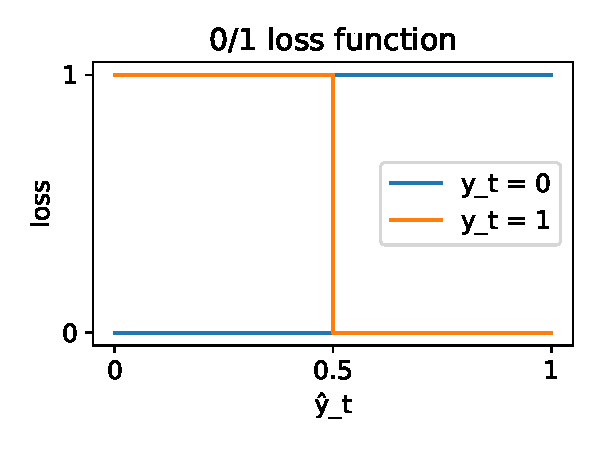
\includegraphics{Pictures/0_1_loss_function.pdf}
  \caption{The 0/1 loss function, shown for both $y_t=0$ and $y_t=1$. It has a
  clear discontinuity at $\hat y_t=0.5$. We can also see from the shape of the
  function that it is not convex.}
  \label{fig:0_1_loss}
\end{figure}


Considering binary classification as a Maximum Likelihood Estimation problem,
we need to assume some joint probability distribution between the features and
the target. A very sensible choice is to assume that the targets are
distributed by a Bernoulli distribution, with a certain probability $p$ of
being the positive class and $1-p$ of being the negative class. The
probabilities of a target being positive or negative for a single observation
$y_t$ in our joint distribution can be dependent on the features of the
observation $x_t$. The likelihood function given a true vector of targets $y$
and a predicted vector of probabilities $\hat y$ is then

\begin{equation}
  \mathcal L(\hat y | y) = \prod_{t}^{T} (\hat y_t)^{y_t} (1-\hat y_t) ^(1-y_t)
\end{equation}

The log-likelihood function then becomes $\sum_t^T (y_t log \hat y_t) + (1-y_t)
log(1-\hat y_t))$, however one models the relation between the features $x$ and
the predicted probabilities $\hat y$. This log-likelihood function is also
known as binary cross-entropy loss, or BCE loss, when negated. This is the most
common surrogate loss function for binary classification. The Binary
Cross-Entropy loss function is theoretically well-founded loss function,
and it also has good gradients for gradient descent. it is also convex, which
gives us convergence guarantees for linear models when performing gradient
descent.

When performing logistic regression, the relation between $\hat y_t$ and $x_t$
is chosen as $\hat y_t = h(w^T x_t)$, where $h : \mathbb R \rightarrow ]0,1[$
is the logistic function $h(x)=\frac{1}{1-e^{-x}}$ that converts odds which
span the real numbers to probabilities in the space $]0,1[$. This then fully
specifies the joint distribution, allowing us to estimate the parameters $w$ of
the distribution.


% The most common surrogate loss function for classification problems is the
% Binary Cross-Entropy (BCE) loss function. This function comes from modelling
% the classification targets as a Bernoulli distribution, investigating $P(y |
% \hat y)$. The log-likelihood function then becomes $(y log \hat y) + (1-y)
% log(1-\hat y))$. 
TODO: REF TRAINING A CLASSIFIER
TODO: CLARITY ABOUT LOSS FUNCTION FOR A SINGLE OBSERVATION / ALL OBSERVATIONS

\subsubsection{Gradient Descent}

We mostly determine parameters for classification and regression models by
solving the empirical risk minimization problem. In the case of least-squares
regression, also known as ordinary linear regression, we are looking for a
function from the family of linear functions from feature space to the real
numbers. The loss function is the square error, which gives rise to the name
"least squares". This optimization problem has an analytical solution, and we
can just set the weights based on this solution. There are many other choices of
both loss function and model function family, though, and most of them do not
have an analytic solution for the weights of the model. Then, we need to solve
the optimization problem in some other way. TODO:REF?

The idea here is that for some families of functions, we can differentiate the
empirical risk with regards to the parameters of the function. This is e.g. true
for the family of linear functions, where we can find the gradient of the
empirical risk given the coefficients of the features as long as we have a
differentiable loss function. We can the follow the gradient backwards towards
the minimum of the function, which is also known as TODO's method in one
dimension, or gradient descent in higher dimensions. I've illustrated the
concept in figure TODO:FIGURE. In every iteration of the gradient descent
algorithm, the parameters of the model $w$ are updated by following the gradient
of the empirical risk $L_w(X,y)$ backwards with a certain step size $\tau$. 

\begin{equation}
  w := w - \tau \nabla_w L_w(X,y)
\end{equation}

Families where we can differentiate the loss function in the parameters are
known as differentiable models. If the loss function is differentiable or even
subdifferentiable, we can perform gradient descent with any differentiable
model. If the empirical risk function is convex in the model parameters as well,
then we can guarantee that following the gradient descent algorithm will
converge to the true minimum of the empirical risk. This is true for any linear
model when using a convex loss function, so using gradient descent for
determining the weights of a linear model guarantees converges.

TODO: REFERENCES

% \subsubsection{Probabilistic Models}
%
% As we have examined Maximum Likelihood Estimation so far, it has been a way for
% us to find a function $f$ that outputs a single value $\hat y_t$ to best
% predict $y_t$. However, Maximum likelihood Estimation doesn't just give us a
% single value, but an entire joint distribution giving us the distribution of
% $y_t$ given $x_t$. This can be used to output not just a single value, but an
% entire probability distribution. 
%
% Classification models e.g. do not usually output just a single class, but
% instead output the probability distribution of the true class being each of the
% possible classes. In the binary classification problem that we have examined so
% far, the model outputs the probability of the true class being the positive
% class along with the probability of the true class being the negative class,
% where the distribution is assumed to be a Bernoulli distribution.
% TODO: REFERENCES

% TODO: EXPLAIN BASED ON MLE
%
% In regression we generally predict a single continuous variable, while in
% classification we predict a single discrete variable. Classification is also
% sometimes used to refer to predicting the probability of an observation
% belonging to different classes, which is an example of what is known as a
% probabilistic model. This is a model that outputs a probability distribution,
% instead of a continuous or discrete prediction, like when we just understood a
% binary classification model as outputting a Bernoulli distribution.
%
% Both classification and regression models can be probabilistic. An ordinary
% linear regression can e.g. be converted to a probabilistic model by outputting
% the prediction uncertainty along with the expected value of the regression
% target, since the model then specifies a normal probability distribution of the
% target.


% \subsubsection{Bayesian Regression}
%
% Probabilistic predictions can often be useful. However, with a trdaditional frequentist approach to MLE, ordinary linear regression gives a centered Gaussian of the same size for every prediction, even though different predictions TODOTODO TODO
%
% Another common example of a probabilistic model is Bayesian regression. In
% Bayesian regression, the parameters of the supervised learning model are
% defined as probability distributions. The parameter distributions can then be
% updated by conditioning on incoming features. Bayesian linear regression is an
% example of a Bayesian regression model.
%
% In Bayesian linear regression, we assume that given coefficients TODO, the
% regression target is distributed by
%
% \begin{equation}
%   y \sim \mathcal N (w^T x, \sigma^2 I)
% \end{equation}
%
%
% Where the $\sigma$ is known as the noise variance, or the amount of variance
% that cannot be predicted by the linear model. We do not know the true
% parameters, and so we assume that the parameters are drawn from some probability
% distribution as well. We ourselves specify some prior probability distribution
% that we can then update by conditioning on new observations using Bayes's rule.
%
% \begin{equation}
%   P(A|B) = \frac{P(B|A)P(A)}{P(B)}
% \end{equation}
%
% TODO: EXPLAIN BAYES'S RULE
%
% Conditioning the model parameters on new data corresponds to what is usually
% known as training a machine learning model. For Bayesian linear regression, TODO
%
% TODO: EQUATION FOR POSTERIOR UPDATE
%
% TODO: BOTH PROBA AND BAYESIAN NEEDS LOTS OF REFERENCES AND LOVE
%
\subsection{Missing Data \& Imputation}

In a machine learning setting, data can be randomly missing. If we go back to
our motivating example for regression, we could for example have failed to
measure TODO. If we want to use a machine learning model that uses a certain
feature as input but the feature is missing for a timestep t, we will have to
somehow deal with the fact that the feature is missing. The data could be
missing from the training dataset, in which case we would either have to remove
that row when training our model, or somehow replace the missing feature with
another value. It could also be missing when we want to make a prediction on a
new observation, in which case we need to replace it with a value to be able to
use our model to generate predictions on this observation. I've illustrated the
different decisions and their outcomes regarding imputing missing data in the
table \ref{tab:imputation}. Even if a model that inherently supports missing
data is used, that model must internally have some method for dealing with
missing data.

\begin{table}
  \begin{tabular}{c|cc}
    & In-sample & Out-of-sample \\
    \hline
    Impute & Skew training distribution & Produce suboptimal prediction \\
    Discard & Do not learn from observation & Produce no prediction
  \end{tabular}
  \caption{Possible solutions to misisng data in the in-sample and out-of-sample case.}
  \label{tab:imputation}
\end{table}

Replacing the missing feature with another value, however it is determined, is
known as imputation. Based on why data is missing, imputation methods can be
more or less appropriate and introduce more or less bias in the data. TODO:REF

\subsubsection{Types of Missing Data}

Missing data mechanisms are classified into three categories:
\begin{enumerate}
  \item MCAR - Missing Completely At Random
  \item MAR - Missing At Random
  \item MNAR - Missing Not At Random
\end{enumerate}

MCAR data is data that is missing independent of the data itself, so the data
loss mechanism has no relation to the data. MAR data is missing dependent on
the rest of the data, but independent of the missing data. This could e.g. be
seen in a survey where male responders might be less likely to report their
income. MNAR data is missing dependent on the missing data. This could for
example be in a system where some values result in errors. Maybe the survey
software doesn't support heights greater than 2m, so these have all gone
missing.

MCAR data has the advantage that it can be reconstructed from joint
distributions between features accurately, with no introduced bias from this
reconstruction. It has the disadvantage that the fact that the feature is
missing carries no extra information, so missing information is non-informative
and only negative for overall model performance.

MAR data can also be reconstructed from joint distributions with present
features without introducing bias, and the missingness can be accounted for
using other present features. The missing information is still non-informative
in this case, though.

MNAR data has the issue that it cannot be accurately reconstructed from present
features, any type of reconstruction will introduce a bias since the missing
data is distributionally different from the present data. However, this also
means that the fact that data is missing is itself informative and can be used
as a feature in the machine learning model.

TODO: REFERENCES
\subsubsection{Imputation Methods}

As mentioned earlier, whenever data is missing, we have the choice of imputing or
discarding it. Imputation can be done based on very simple best guesses based
on historical observations of the feature, all the way up to quite complex
model-based imputation methods using present features and statistical methods.
Some common imputation methods are:

\begin{enumerate}
  \item Mean/Mode Imputation
  \item Using Domain Knowledge
  \item Tabular Supervised Learning Models
  \item Fully Conditional Specification
\end{enumerate}

1) Mean/mode imputation replaces the missing value with the historical mean or
mode of the feature. This is simple and practical but might considerably
skew the distribution. Nonlinear supervised learning methods can
significantly deteriorate if mean/mode imputation is used in the training
set due to the change of the feature distribution. TODO: REF

2) Sometimes, domain knowledge can be used to reconstruct missing data. This is
usually in situations with either MAR or MNAR data. TODO:EXAMPLE

3) Tabular supervised learning models, e.g. k-nearest-neighbors or random
forest, can be used for reconstruction, by training on historical data and
reconstructing missing data using it. This allows capturing quite complex
relations between data, but pushes down the problem of imputation another
step, since these regressions will then also need to somehow deal with
missing data.

4) Fully conditional specification is a specific way of using tabular
supervised learning models that deals with the issue of imputing missing
input features for the imputing models. It is further explained in section
TODO.

\subsubsection{Fully Conditional Speciication}

Fully conditional Specification (FCS) is a method of imputing missing features
based on present features. It defines for every feature an imputation model
based on the other features. An imputation model is literally a supervised
learning model, that takes the other features as inputs and spits out the
imputed feature as the output. One algorithm for FCS is known as the
Mutlivariate Imputation by Chained Equations (MICE) algorithm, which is a
Markov chain Monte Carlo method, meaning that it is a probabilistic process
where every step is only dependent on the previous step.

The algorithm works by first filling in every missing data point with a random
value that the feature has taken on before TODO:IN THE TRAINING DATASET. The
algorithm then goes through and trains for each feature an imputation method,
and the method predicts the missing values of that feature using its imputation
method. The algorithm supports defining a probabilistic imputation method, in
which case a value is drawn from the imputed distribution.  TODO: DOES THE
MODEL TRAIN ON ALL VALUES OR ONLY THE ONES THAT WERE ORIGINALLY PRESENT? This
is done recursively a few times, which ends up giving a value for every missing
feature. Since this is a probabilistic process, it can be sampled several times
to get both a more accurate estimate of the imputed feature, as well as a
probability density for it.

Fully Conditional Specification is flexible and simple to use but can be quite
computationally expensive, since it requires training many imputation models
several times and the entire algorithm needs to be run several times to reduce
sampling error. TODO: GIVE REASON FOR PRESENTING FULLY CONDITIONAL
SPECIFICATION

TODO: THE ALGORITHM WORKS ON THE ENTIRE TRAINING SET IN ONE GO
TODO: REF STEPH VAN BUUREN
TODO: THIS SHOULD BE SOMEHOW COMPARED IN THE RESULTS

\subsection{Online Learning}

Online learning is as mentioned earlier a different method of machine learning
than the tabular learning approach. In online learning, observations and
targets come in a streaming fashion, and the model must be updated in an
iterative way.

Parameter learning must be done differently in online learning, since not only
the parameters found are important, but also how rapidly they can be found. If
a model e.g. has extremely poor loss all the way until the final observation,
whereafter it becomes amazing, it does not perform very well for an online
learning task. To quantify this requirement in online learning, we introduce
the term regret.

Regret is a term that comes from adversarial game theory. I'll explain it using
an example. Imagine that you're playing a game against an adversary where he is
secretly deciding on a random number between 0 and 1 every round of the game.
You then want to decide on some number for your guess on every round. Then,
every round, you experience a loss equal to the squared distance between your
guess and the true value of the random number. Your regret is then the
difference between the sum loss you experienced, and the sum loss experienced
by the best choice you could have made.

Within this concept of minimizing regret, we can return to our world of
supervised learning. Then, the regret is the difference in cumulative loss
between our model and the best possible choice of model parameters. In online
learning situations, TODO REGRET MINIMIZATION AND SUBLINEAR REGRET TODO I'M NOT
USING THIS THEORY YET

Online learning methods are usually based on some iterative updating of a set
of model parameters, sometimes one time step at a time, and sometimes in a set
of small batches. TODO:REF

Online linear regression is quite simple, and is seen already in TODO:FIND REF.
Online linear regression can be performed in two separate ways. One method is
to continuously update the matrix $X^TX$, to then invert it every step and use a
newton-Raphson step to update coefficients at every iteration. Another method
is to update coefficients using a coordinate gradient descent step.

TODO: I'M NOT TALKING ABOUT REGRET ANYWAY??

\subsubsection{Stochastic Gradient Descent}

Supervised learning problems generally involve minimizing some loss function
over a dataset. In online learning, we don't have access to the entire dataset
at once, and instead receive one observation at a time. We want to minimize
regret for the model we choose based on this observation. We can do this using
a variant of gradient descent known as stochastic gradient descent.

In batch learning, we have access to the entire dataset simultaneously and can
compute the gradient of the loss function with regards to the model across the
entire dataset. We can then update the parameters by moving along the negative
gradient. This is known as gradient descent. In online learning, we can instead
compute the gradient over one observation at a time and see this gradient as an
estimate of the true gradient. We can then update our model parameters based on
this estimated gradient. Due to the noisiness of the estimation of the
gradient, this algorithm is known as Stochastic Gradient Descent.

TODO: SHOW EQUATIONS ALSO

Stochastic gradient descent lets us bound the regret of our model choice if we
can bound the variance of the estimated gradient and choose our step sizes
well. It is then an obvious method for updating a supervised online learning
model and is the only method we will see in this thesis for updating model
weights.

\subsubsection{Evolving Feature Space}
So far, we have always thought of our data as having a fixed set of features,
the feature space. We start out expecting that all features are there, and
whenever a feature is not there, we think of it as “missing” and reconstructing
it is then known as “imputing” this feature. In machine learning generally and
especially within online learning, it sometimes makes sense to think of feature
spaces as evolving over time. Instead of saying that we have a fixed set of
features over time, we instead have a set of features at every time step, and
that set of features changes over time. As I discussed in the introduction,
this is especially sensible when considering features from a conglomerate of
real-life entities.

The dynamics of feature spaces can be understood by considering the following
four events that happen over the course of a feature's evolution.
\begin{enumerate}
  \item The feature appears for the first time.
  \item The feature is observed normally at a time step.
  \item The feature is randomly missing at a time step.
  \item The feature disappears forever.
\end{enumerate}

Events 1 and 4 only happen one time each, while events 2 and 3 can both happen
an arbitrary number of times. TODO: IS THIS MENTIONED ANYWHERE IN LITERATURE?
This taxonomy explains the dynamics that a model designed for variable feature
space must deal with.

While this taxonomy is useful, there is an issue with it. From the point of
view of the model, there is no difference between a feature that is randomly
missing and a feature that has disappeared permanently. In a non-stationary
environment, a feature that has been missing for a long time might suddenly
appear again but now have a completely different effect in the context of the
model. Then, it might be better to think of this as a different feature. In
this light, it might make sense to let a feature disappear from the knowledge
of the model once it has been gone for long enough, thus setting a cutoff point
for when the feature is missing. TODO: CONFUSING

TODO: FIGURES

\subsection{Marginalizing and Conditioning}
TODO: MARGINALIZING AND CONDITIONING

\subsection{Utilitarian Online Learning}
The name Utilitarian Online Learning (UOL) refers to online learning methods
that work with evolving feature spaces, and was introduced by the survey
article TODO. The goal of utilitarian online learning models is not simply to
produce the best predictions within this space, but also to be computationally
efficient.

The survey artice presents six state-of-the-art utilitarian online learning
models. It also introduces a taxonomy of current utilitarian online learning
models based on their approach to evolving feature space and their model of the
setup. It splits models into three categories: 

\begin{enumerate}
  \item Passive-Aggressive
  \item Feature Correlation
  \item Evolutionary Ensembles
\end{enumerate}

Passive-Aggressive methods work by waiting to incorporate new features into
their predictions until they have been present for a while. Feature Correlation
methods work by reconstructing missing features using some relation between
features when they were observed. Evolutionary Ensembles work by evolving a
nonlinear ensemble of weak classifiers, typically a forest of decision trees.
Two models are presented in every category, and all models are classifiers.
While they have been tested on some datasets, one issue in this survey article
is the relative lack of clarity regarding when to use which of these models.

I will now introduce some models from the literature that we will touch on
again later, some in depth and some less so. While I spend some time
introducing them here, we will see in the results section that we are going to
want to develop a new model, as these models either do not perform or do not
perform very well. They are also all classifiers, and regression is a more
natural forecasting task in our intended application space.

\subsubsection{Online Linear Model (OLM)}

One of the simplest ways to model regression is with a linear model. Ordinary
linear regression is the most common, but statistics has a whole set of
possible linear regressors that arise when choosing different joint probability
distributions and performing maximum likelihood estimation for their
parameters.

The Online Linear Model, or OLM, is a way to implement linear models in a
utilitarian online learning context. The model is first introduced in the paper
TODO, where it is termed the Online Convex Optimization method. Here, they use
it as a linear classifier, but they don't present the exact workings of the
model, since they only use it as a baseline.

An online linear model can be implemented with any joint probability
distribution between the targets and features. I specifically implement two
variants, one for regression and one for binary classification, i.e. with the
joint probability distributions specified as $y_t$ normally distributed around
$w^T x_t$, and $y_t$ Bernoulli distributed with probability $h(w^T x_t)$,
respectively. For both implementations, the baseline online linear model will
handle missing features by mean imputing them. I assume centered input
features, which means that mean imputing missing features will be the same as
setting them to zero. This will be useful for the implementation of the model.

The OLM has a set of weights $\mathbf w$, one for every input feature seen up
to time $t$. This space of all observed features up until time $t$ is known as
the universal feature space, $u_t$. At every time step $t$, it receives some
features $\mathbf x_t$. All features are not necessarily present. The set of
present features is denoted $d_t$.

The idea of the model is then to receive the features for a time step, and
producing predictions based on only the present features, zeroing out missing
features which is the same as mean imputing them. The weights are then updated
based on only present features. Whenever a new feature appears, it is given a
new weight that is initialized to zero. The general function of the model is displayed
in figure TODO: INSERT FIG.

For the regression variant assuming that $y_t$ is normally distributed around
$w^T x_t$ with some noise variance, the prediction $\hat y_t$ is given by

\begin{equation}
  \hat y_t = \sum_{i \in d_t} w_i x_i + \sum_{i \in (u_t \backslash d_t)} w_i 0 = \bar{\mathbf{w}}^T \mathbf {x_t}
\end{equation}
Here, $\bar{\mathbf{w}}$ is the set of weights for present features,
$\bar{\mathbf{w}} = [w_i \text{ for } i \in d_t]^T$.

The weights are then updated using stochastic gradient descent. The loss
function is the mean square error, meaning that the loss observed at a single
time step will be $l(\hat y_t, y_t) = (\hat y_t - y_t)^2$. The gradient descent
update step is then given by following the negative gradient of the loss
function with regards to the weights of the model

\begin{equation}
  \nabla_w ( \bar{\mathbf{w}}^T \mathbf {x_t} - y_t)^2 = 2 x_t(\bar{\mathbf{w}}^T \mathbf {x_t} - y_t)
\end{equation}

This gives us the update step
\begin{equation}
  w := w - \tau 2 x_t(\mathbf{w}^T \mathbf {x}_t - y_t)
\end{equation}
where $\tau$ is a step size parameter which I will discuss further in the
section TODO. Since missing features have values of $x_t=0$, they will not be
updated, and the update step can be written in a more efficient form as
\begin{equation}
  \bar w := \bar w - \tau \, 2 (\bar {\mathbf{w}}^T \bar {\mathbf {x}}_t - y_t) \bar {\mathbf{x}}_t
\end{equation}

\textbf{Classification variant} TODO: FIGURE OUT SUBSECTION DEPTH OF THIS

The classification variant works mostly in the same way. The prediction is
formed as

\begin{equation}
  \hat y_t = h(\sum_{i \in d_t} w_i x_i + \sum_{i \in (u_t \backslash d_t)} w_i 0) = h(\bar{\mathbf{w}}^T \mathbf {x_t})
\end{equation}
where $h$ is the logistic function, $h(z)=\frac{1}{1-e^{-z}}$.

Again, weights are updated using stochastic gradient descent. The loss function
for the classification model is the loss function attached to the Bernoulli
joint probability distribution, which is the binary cross-entropy (BCE) loss,
as you might remember from section TODO: REF. The loss is then $l(\hat y,y) =
(y_t log \hat y_t) + (1-y_t) log(1 - \hat y_t)$ for a single time step. The
objective function written for a single time step is then

\begin{equation}
  \mathcal F = -(y_t \text{log} \hat y_t) + (1-y_t) \text{log}(1 - \hat y_t) 
\end{equation}

Since $\hat y_t = h(w^T x_t)$, we can split the gradient up into a couple of
factors using the chain rule. We'll define $z_t = w^T x_t$, and the partial
derivative for parameter $w_i$ will then be given by 

\begin{equation}
  \frac{\partial \mathcal F}{\partial w_i} = {\partial \hat y_t}\frac{\partial
  \mathcal F}{\partial \hat y_t} \cdot \frac {\partial \hat y_t}{\partial z_t}
  \cdot \frac{\partial z_t}{\partial w_i}
\end{equation}

The three factors are found:

\begin{equation}
  \frac{\partial \mathcal F}{\partial \hat y_t} = -(\frac{y_t}{\hat y_t} - \frac{1-y_t}{1-\hat y_t}) = -\frac{y_t - y_t \hat y_t + y_t \hat y_t - \hat y_t}{\hat y_t (1 - \hat y_t)} = -\frac{y_t - \hat y_t}{\hat y_t (1 - \hat y_t)}
\end{equation}
\begin{equation}
  \frac{\partial \hat y_t}{\partial z_t} = \nabla_{z_t} \frac{1}{1 - e^{-z_t}} = \frac{-1}{(1 - e^{-z_t})^2} \cdot (-e^{-z_t}) = \frac{e^{-z_t}}{(1-e^{-z_t})^2} = \hat y_t (1 - \hat y_t)
\end{equation}
\begin{equation}
  \frac{\partial z_t}{\partial w_i} = \frac{\partial}{\partial w_i} w^T x_t = x_i
\end{equation}

The partial derivative for $w_i$ is then

\begin{equation}
  \frac{\partial \mathcal F}{\partial w_i} = -(\frac{y_t - \hat y_t}{\hat y_t (1 - \hat y_t)}) (\hat y_t (1 - \hat y_t)) (x_i) = x_i(\hat y_t - y_t)
\end{equation}

and the gradient becomes $\nabla_w \mathcal F = x_t (\hat y_t - y_t)$. Again,
the gradient for any missing feature will be zero, and they can be left out of
the update. the update step for the classification version of the online linear
model is then given by

\begin{equation}
  \bar w = \bar w - \tau \bar x_t (\hat y_t - y_t)
\end{equation}

The model deals with new features by initializing their coefficients to zero.
The vector of parameters $w$ can thus grow over time. The algorithm pseudocode
for the online linear regression model is shown in algorithm \ref{alg:olm}. The
runtime complexity for a single time step is of order $O(d_t)$. The memory use
is of order $O(u_t)$. The model is thus a useful baseline model to compare to,
since it runs in linear time and is lightweight. 

\begin{algorithm}
  \caption{Online Linear Model - Regression}\label{alg:olm}
  \begin{algorithmic}
    \State Initialize empty weights vector $w$
    \For{$t \in \{0,1,\dots,T\}$}
      \State Receive $x_t$ with present feature set $d_t$.
      \State Initialize unseen features, $w_i := 0 \,\, \forall i \in \{d_t - u_{t-1}\}$.
      \State Predict $\hat y_t = \bar w^T x_t$
      \State Update $w$, $\bar w := \bar w - \tau\, 2 x_t (\hat y_t - y_t)$
    \EndFor
  \end{algorithmic}
\end{algorithm}

\subsubsection{OCDS}

The Online Learning on Capricious Data Streams (OCDS) algorithm is a linear
classifier, and a feature correlation method in the categorization from
TODO:REF. It reconstructs missing features by averaging the expected value of
the feature given the set of present features. 

If e.g. feature $j$ is missing, it is reconstructed as $x_j =
\frac{1}{d_t}\sum_{i \in d_t} \mathbb E \lbrack x_j | x_i\rbrack $. Since it is
assumed that features are drawn from a normalized multivariate normal
distribution, the expected value of one feature given another is given by the
function $\mathbb E \lbrack x_j | x_i \rbrack = \Sigma_{i,j}x_i$. These
coefficients are stored in a matrix G, $\mathbb E \lbrack x_j | x_i \rbrack =
\Sigma_{i,j}x_i$. This is the basic idea, where $G$ can then be found by
minimizing the reconstruction error $\|G x_t - x_t\|$ TODO: PROJECTION, but the
paper then introduces some regularization on the matrix as well, as well as
adding a term based on the true regression targets.

The model ensembles predictions based on reconstructed features and present features together TODO

The OCDS model takes some unorthodox decisions in its implementation. I have
further on discussed the OCDS model, see section TODO: DISCUSSION OF OCDS
SECTION. 
TODO: NORMALIZED VS STANDARDIZED VS CENTERED.

\subsubsection{OLVF}

The Online Learning from Varying Feature Spaces (OLVF) algorithm is also a
linear classifier, classified as a passive-aggressive learner in the taxonomy
from TODO. It deals with missing features by projecting observed features into
a shared subspace with the classifier itself. The model minimizes a hingle loss
with slack, which turns out to have some complications regarding markets as
will be discussed later TODO:THIS REQUIRES MARKET PARTICIPANTS TO PAY FOR
SLACK.

\subsubsection{OVFM}
The Online Learning in Variable Feature Spaces with Mixed Data (OVFM) algorithm
is also a linear classifier. It is a development of OCDS and works generally the
same way. The main difference is that it uses Gaussian copula to map features
into a latent space and performing classification in this space. This allows
for better gradients when dealing with ordinal features. TODO:WHY?

\section{Game Theory}

Game theory is the study of strategic interactions between rational agents. Put
another way, game theory is the study of how agents will interact if every
agent in the game is acting to optimize some measure of personal gain. An
interaction between rational agents is known as a game. 

The first issue in game theory is then to quantify this personal gain. We
assign a mathematical value to the preference of agents, known as their
utility. The agent prefers the outcome with a higher utility to the outcome
with a lower utility, and they'll act to maximize their utility. In many cases,
the utility represents the monetary value of an outcome to an agent. Therefore,
the utility of an outcome is also often known as the payoff of the outcome.

A game has a set of possible outcomes O. Every agent $i$ has a set of
strategies they can choose between, known as their strategy space, $S_i$. The
outcome can be represented as the set of chosen strategies of every agent, $O =
{S_1,S_2,\dots,S_n}$. When we investigate how agents act in a game, we assign
them a utility function that maps an outcome to the real numbers $f: O
\rightarrow \mathbb R$. The output is the utility. A note about naming: I will
use the words agent, player, and participant interchangeably in referring to
the agents in a game theoretical game.

\subsection{Nash Equilibrium}
We define within the study of a game the concept of equilibrium. An equilibrium
is some point in the strategy-space of a game that fulfills a set of
equilibrium conditions. The most studied equilibrium is the Nash equilibrium,
which is characterized by no agent being able to change their strategy and
improve their payoff, given that all other agents retain their current
strategies.

%TODO:EXAMPLE?

We generally assume that games end up at a Nash equilibrium, since at every
other point in the game, at least one agent is incentivized to change their
strategy. When we talk about a game being in equilibrium, we are therefore
referring to it being in a Nash equilibrium.

%TODO: SOCIAL UTILITY MAXIMIZATION AND REVENUE MAXIMIZATION

\subsection{Individual Rationality}

When we are investigating a game, we might characterize it by certain
properties that it holds at equilibrium. One concept that we might be
interested in is whether participants want to participate in the game or would
rather abstain as they might be able to in some situations. Since we expect all
games to move towards the Nash equilibrium, we want to know if in the Nash
equilibrium, every player experiences a higher payoff by participating in the
game than they do from abstaining. Understanding payoff as monetary value, we
can define the payoff of abstaining from the game as 0. Then, we can say that a
game is individually rational if every player has a non-negative payoff in the
Nash equilibrium $o$, $f_i(o) \geq 0 \,\, \forall i$. Players are willing to
participate in individually rational games.

\subsection{Bayesian Games}
A Bayesian game is a game where the agents do not have complete information at
the outset of the game. This means that they cannot independently assign an
exact payoff to every outcome of the game. In a Bayesian game, each agent has
some private information known as their “type”. This makes it sound like their
private information is somehow a discrete class, but private information can be
anything, including a continuous value. Private information effectively
introduces a probabilistic element into a game from the point of view of the
agents, since their valuations of a good are no longer exact and depend on
their beliefs about the private information of other agents, and these
valuations can be represented as probability distributions.

TODO: BETTER UNDERSTAND AND EXPLAIN THE DIFFERENCE BETWEEN NORMAL AND BAYESIAN GAMES

In a Bayesian game, we no longer call the equilibrium the Nash equilibrium.
Instead, we introduce the Bayesian Nash equilibrium. It is characterized by a
point where no participant can increase their expected payoff given the
strategy of the other participants. The difference between a Nash equilibrium
and a Bayesian Nash equilibrium is that we now consider the property in
expectation, instead of deterministically.

\subsubsection{Example: Second Price Auction}

Auctions can be understood as game theoretical games. A classic auction that is
easily understood is the second price auction. The process of the second-price
auction is as follows:

\begin{enumerate}
  \item Each participant bids on the good in a sealed bid.
  \item The participant with the highest bid pays the second-highest bid for
    the good.
\end{enumerate}

In the complete information variant, where every participant knows ahead
of time their exact valuation of the good, the Nash equilibrium is every bidder
bidding their private valuation. This equilibrium is individually rational.

One can specify many different Bayesian variants of the Second Price Auction
where the auction mechanism is the same, but the information and valuations for
the sellers are different. One version is a common value action. In a common
value auction, there is only one true valuation of the good, and every bidder
has their own signal for what this true valuation is. Signals come from a joint
probability distribution.

Now, let's say that we have a good with a true valuation of $v=100€$, and every
bidder $i$ receives a signal on the price equal to $v_i = 100€ + \epsilon_i,
\epsilon_i \overset{iid.}{~} \mathcal N(0,\sigma^2)$. We have at least four
bidders. Then, if every bidder bids their signal directly, the winner will be
likely to have bid too much for the item and end up paying more for the good
than they value it for.

This is obvious if we consider a situation with just four bidders. When we have
four bidders, both the highest and the second-highest bid will be greater than
the mean in expectation. TODO: MATH OR REF FOR THIS Since the mean is the true
valuation, the highest bidder will pay more than their true valuation for the
good. They will thus come out of it with a net negative utility. This is where
the term \emph{winner's curse} comes from TODO:REF, since many real-world goods
are valued at least partially by a common value, so directly bidding your best
guess for the value of a good will be likely to end up in an overall loss.

The best bid is instead bidding strategically based on your own signal and your
estimated joint probability distribution with the other bidders' signals. This
is known as strategic bidding and can quickly become complicated.
In this case, solving the optimal bidding problem requires finding the
expectation TODO, which is the expected true valuation of the good given your
own signal and conditional on all other bidders having a signal less than
yours, which is already a complicated calculation even for this simple auction.

TODO: REF AUCTIONS.PDF FROM MY DRIVE
TODO: SHOULD I DO LIKE EXAMPLE BOXES?

\subsection{Bayesian Game Properties}

From the second-price auction example, we see a new effect in Bayesian games.
We can encounter situations where agents have some private information but are
incentivized to report some different information to the other participants in
the game. In auctions, this is known as strategic bidding, and it can make
bidding well in an auction a complicated and computationally expensive process.
A desirable property for a market is then that the optimal decision for all
participants is to bid their private information, i.e. bidding your private
information is a Bayesian Nash equilibrium point. This is known as the market
being \emph{truthful}.

We also have to reexamine our definition of individual rationality. Before, we
defined it based on the outcome in the Nash equilibrium. In a Bayesian Nash
equilibrium, we have two points in time from which we can see this outcome: In
expectation before the game is finished, or after the game is finished known as
ex-post. A game can have a positive expected payoff, but still give a negative
payoff in a specific shot of the game. This gives rise to two different
versions of individual rationality: one that holds in expectation, and another
that holds in every single run of the game in the Bayesian-Nash equilibrium,
known as Ex-Post Individual Rationality (EPIR). An EPIR game is also
individually rational in expectation, but a game that is individually rational
in expectation is not necessarily EPIR.

While truthfulness is only a single property, since it is a property of games
with private information, many properties for Bayesian games have a stronger
ex-post variant and a weaker in-expectation variant. This will also be true for
properties defined in TODO:REF related to fair revenue distributions to
multiple sellers in an analytics market.

\subsection{Cooperative Game Theory}

Cooperative game theory is a branch of game theory in which players can make
binding agreements externally to the game, allowing players to join forces as
groups known as coalitions. A cooperative game is concerned with the sum payoff
for a coalition, and can be defined by a characteristic function $v: 2^N
\rightarrow \mathbb R$ from a coalition $\omega$ of players to a sum payoff
$v(\omega)$. The coalition of all players is known as the grand coalition.

%TODO: REF https://vknight.org/Year_3_game_theory_course/Content/Chapter_16_Cooperative_games

Cooperative game theory also answers the question of how to fairly distribute
the payoff of a cooperative game, using a specific definition of fairness. This
payoff distribution is known as the Shapley value, named after economist Lloyd
Shapley. Fairness is understood by examining the effect of adding a player to a
coalition, and examining how adding the player increases or decreases the sum
payoff. Specifically, it guarantees what is known as Shapley fairness, which is
the following properties:

\begin{enumerate}

  \item Balance - The total payoff from the grand coalition is distributed,
    TODO: EQUATION

  \item Symmetry - If two players have the same effect in all coalitions, then
    they receive the same portion of the total payout. Basically, the way we
    order our players does not matter.

  \item Zero Element - If a player has no effect on any coalition, then they do
    not receive any payoff.

  \item Additivity - If we have two cooperative games and add them together,
    the sum payoff for each player is the sum of their payoff in the first game
    and their payoff in the second. I.e. how the payoffs are distributed is the
    same whether we examine the games individually or as a single game.

\end{enumerate}

These are the fairness properties that are guaranteed by the Shapley value. The
Shapley value turns out to be the unique way to distribute payoffs that
guarantees these properties. It is calculated by examining the effect of adding
a player to every possible coalition that it isn't already in. The equation for
the Shapley value $\psi_i$ for player $i$ in the game given by characteristic
function $v(\omega)$ is calculated from the following equation:

\begin{equation}
  \psi_i = \sum_{S \subseteq N \backslash \{i\}} \frac{|S|!(n-|S|-1)!}{n!} [v(S \cup \{i\}) - v(S)
\end{equation}

Here, $S$ is a coalition, and $N$ is the set of all players. $N \backslash
\{i\}$ is then the set of all players except player $i$. $n$ is the total
number of players. The equation then calculates for every coalition $S$ the
difference between the payoff when $S$ does and does not contain $i$, and
averages this by how many orderings exist of this coalition. The Shapley value
can be seen as a function from a characteristic game to the contribution of
every participant to the overall payoff of the game. It is also used in e.g.
machine learning to explain the contribution from every input feature to an
output. TODO:REF

\subsection{Analytics Markets}

An analytics market can be seen as a game. It contains two classes of agents,
buyers and sellers, and they interact with the market in different ways. The
analytics market was as mentioned earlier formalized in TODO:REF AGARWAHL. The
formalization in this thesis is slightly different, and can be seen in the
figure TODO:REF FIG IF I WANT A FIGURE HERE.

While I only investigate the seller side of the market, there is already
well-founded solutions on the buyer side to incentivize truthful bidding for a
data buyer in the market. TODO:REF

Though a market can have several buyers, we can clear the market separately for
each buyer. We then always consider a market with a single buyer, and call that
buyer the \emph{central agent}, and every other participant in the market
selling features we term a \emph{supporting agent}. The central agent will
themselves bring some features to the table. The set of features belonging to
the central agent is called $I_c$.


When determining the payoff, we only care about reduction in the loss function
below what the central agent loss would be with only their own features. We
then let the revenue $\pi_t$ for the central agent for time $t$ be given by
TODO: DECIDE ON NOTATION FOR GAIN FUNCTION, AND CONSTRAINTS ON GAIN FUNCTION

\begin{equation}
  \pi_{\omega,t} = G(l_{\omega_c, t} - l_{\omega, t})
\end{equation}

Where $\omega_c$ is the features belonging to the central agent, and $\omega$
is some coalition. The market uses the Shapley value based on this
characteristic function to distribute the revenue between sellers. We get a sum
flow of revenue $\pi_{\Omega,t}$ from the central agent to the supporting agents through
the market, where $\Omega$ is the grand coalition.

\subsubsection{Market Properties}

We want our market to fulfill a number of properties for the incentives of the
feature sellers. We want the revenue distribution to be fair according to the
Shapley fairness criteria, as listed above, as well as truthful and
individually rational in expectation. However, in an analytics market, we
cannot guarantee anything about the out-of-sample distribution. The
out-of-sample distribution might drift, which happens regularly in real-world
machine learning tasks TODO:REF. Therefore, we instead look at the properties
of the market if applied in-sample. While this is a fictitious situation, see
section TODO:INSAMPLE SECTION, there is currently no work on proving properties
in the out-of-sample situation, so we must limit ourselves to in-sample
properties.

Looking at the market in-sample, we then investigate the point that our
regression mechanism converges to. In this situation, the four Shapley criteria
come directly from using the Shapley value as the revenue distribution policy.
Individual rationality and truthfulness cannot be guaranteed for an arbitrary
regression mechanism. I will discuss truthfulness in section TODO: REF SECTION,
since we also need to define exactly what truthfulness means in terms of an
analytics market.

Individual rationality requires that every participant expects positive
returns. Let us consider a linear model with weights $w$ that minimizes a
convex loss function $l$.

\begin{equation}
  \underset{w}{\text argmin} \mathbb E \lbrack l(X w - Y) \rbrack 
\end{equation}

Where $X$ and $Y$ are the in-sample features and targets, respectively. It is
well known that adding an additional feature to this setup will always reduce
the loss or keep it constant. Therefore, the difference in payoff used to
calculate the Shapley value will always be positive, so the Shapley value
itself will always be positive, and thus any seller expects positive revenue
in-sample, and the market is individually rational.


% The figure shows the divisions of the analytics market. The buyers receive
% prices and produce bids in the form of supervised learning targets and a
% willingness to pay $G : \mathbb R -> \mathbb R$ for a certain decrease in their
% experienced loss. specify to the market their supervised learning task, as well
% as how much they would earn from a certain increase in predictive performance.
% TODO: REF AGARWAHL produce a method of pricing and prediction that is truthful
% in expectation, i.e. buyers are incentivized to provide their true supervised
% learning targets and willingness to pay and cannot earn more e.g. by scaling
% back on how much they are willing to pay for a prediction increase. TODO: WHY?

% Sellers on the other hand provide the market with features. Features are used
% in a supervised learning method, regression or classification, for training and
% prediction to produce predictions for the buyers in the market. The payment
% from buyers is then distributed among sellers according to the revenue
% distribution function. The revenue distribution function is calculated using
% the Shapley value. The cooperative game is a game where the players are
% prediction features and the outcome is prediction performance as expressed by
% the willingness to pay function from the buyer. The Shapley
% value then fairly distributes the revenue from the buyer between the features
% owned by the sellers, determining the payout for each feature.

% The market mediates the features of the sellers and the prediction tasks of the
% buyers by use of a regression mechanism. To ensure the properties of the
% market, this regression mechanism needs to have some specific characteristics.


% TODO: I MIGHT NOT WANT TO DO THE INFORMATION THING, ITS A WHOLE SILLY COMPLICATION. I CAN JUST DO A PROBABILITY BASED LOSS FUNCTION.
% The above method for revenue distribution is the maximum likelihood variant of the market. TODO:REF FALCO also brings analytics markets to probabilistic models, where the KL divergence is used to measure the information added by features in the market. The characteristic function changes in this case, 
% TODO: PROBABILISTIC MARKET
% TODO: EXPLAIN THAT THIS IS MAXIMUM LIKELIHOOD APPROACH



\subsubsection{Truthfulness}

We want our market to incentivize the sellers to truthfully report their
features, but first we must define what truthfulness means in an analytics
market. We define truthfulness as the property that any market participant
maximizes their expected returns by reporting their features without adding
centered gaussian noise. Any other transformation we understand as feature
engineering, which we allow agents to do freely. This is sensible, since the
agents might have features in any representation, and if another transformation
of their information increases the prediction quality of the market, that
should not be disincentivized

TODO: REF AGARWAHL assume that the prediction model is of a type where adding
gaussian noise to input features does not increase prediction accuracy. TODO:
REF PINSON shows that this assumption holds in-expectation in-sample for any
linear model that minimizes a convex loss function when the Shapley value is
used for revenue distribution, and the buyer's willingness to pay function is
itself a monotone decreasing function in the loss function.

\subsubsection{Robustness to Replication}

Unfortunately, there is an extra complication to this story. Fairness is
ensured at the feature level, and therefore does not guarantee that everything
is fair at the seller level. If several sellers have correlated features, one
seller might duplicate their feature, selling it twice in the market. This saps
away the payoff from other sellers to the malicious seller. A revenue
distribution mechanism that doesn't have this attack vector is known as robust
to replication, and while there are attempts to solve the problem of
replication robustness, it is an open problem within the field of analytics
markets.


\subsubsection{In-Sample Markets}

Other literature on analytics markets present in-sample markets, where
participants pay for in-sample performance along with out-of-sample
performance. This makes market properties more sensible, since generally,
market properties cannot be guaranteed to hold out-of-sample in non-stationary
data where the underlying distribution might not be the same as in the
in-sample data. In some way, paying for in-sample performance makes sense, as
it is at prediction time a useful measure for the predictive capabilities of
your model.

Since in a real market, participants are not actually interested in the
in-sample performance, but instead the out-of-sample performance, I have
decided not to include the in-sample market in this thesis. While I mentioned
before that in-sample performance is a useful measure, it is also not the best
measure for performance. For many applications a set of hold-out data will be
used to evaluate the model. This data is known as either test or validation
data depending on the exact use, and is a better measure of model performance
than the in-sample loss. TODO:REF.

While the properties of the market are only guaranteed in-expectation
in-sample, I still argue that leaving out the in-sample market is more
appropriate as all users of the market only care about out-of-sample
performance. We assume the out-of-sample distribution to be similar enough to
the in-sample distribution that training on in-sample data is sensible;
otherwise, the entire analytics market is itself useless.
